\section{Theoretische Grundlage}
\label{sec:Theorie}
\subsection{Ziel}
Ziel des Versuches ist es die elastischen Module eines Metalls und das magnetische Moment eines Permanentmagneten mittels einer Drehschwingung zu bestimmen.
\subsection{Normal-, Schubspannung und Hooksches Gesetz}
Kräfte die an die Oberfläche eines elastischen Körpers angreifen, verformen diesen. Aufgrund dessen wird die Größe Spannung definiert, welche ein Verhältniss von der Kraft zu einem Flächenelement herstellt.
\begin{equation}
  \sigma = \frac{Kraft}{Fläche} = \frac{\text{N}}{m^2}
  \label{eqn:Spannung}
\end{equation}
Sie lassen sich in zwei Kategorien aufteilen. Als Normalspannung $\sigma_\text{N}$ werden die Kräfte bezeichnet welche senkrecht zur Oberfläche stehen. Die Kräfte welche parallel zur Oberfläche stehen heißen Schubspannung $\sigma_\text{S}$. Desweiteren gibt es noch Volumenkräfte. Bei solchen greift die Kraft an jedem Volumenelement an, zum Beispiel die Schwerkraft.

Zwischen hinreichend kleinen Spannungen und Deformationen besteht ein proportionaler Zusammenhang welcher als Hooksches Gesetz bezeichnet wird.
\begin{equation}
  \sigma = E \frac{\Delta L}{L}  \hspace{2em} \text{und} \hspace{2em} P = Q\frac{\Delta V}{V}
  \label{eqn:Hook}
\end{equation}
Um alle Spannungen in einem Kristall vollständig zu beschreiben werden jeweils sechs Komponenten benötigt, wobei drei für die Gestalts- und drei für die Volumenelastizität zuständig sind. Bei einem einfachen  Kristall mit niedriger Symmetrie entsteht deswegen eine 6x6-Matrix mit 36 Einträgen. Bei kubischen Kristallen lassen sich aufgrund der Symmetrie der Matrix und des Körpers die Einträge auf 3 verringern. Handelt es sich zusätzlich um einen isotropen Körper, so lässt sich der Körper vollständig durch 2 Konstanten beschreiben.

\subsection{Elastische Konstanten isotroper Stoffe}
Zur Berechnung der elastischen Konstanten wird einerseits der Torsionsmodul $G$, als auch der Kompressionsmodul $Q$ benötigt bzw. der Elastizitätsmodul $\sigma$.
Die Poissonsche Querkontraktionszahl $\mu$ verknüpft die Längenänderung mit der Normalspannung. Die Abbildung \ref{fig:poisson} soll dies anhand eines einseitig eingespannten Stabes verdeutlichen.
\begin{figure}
  \centering
  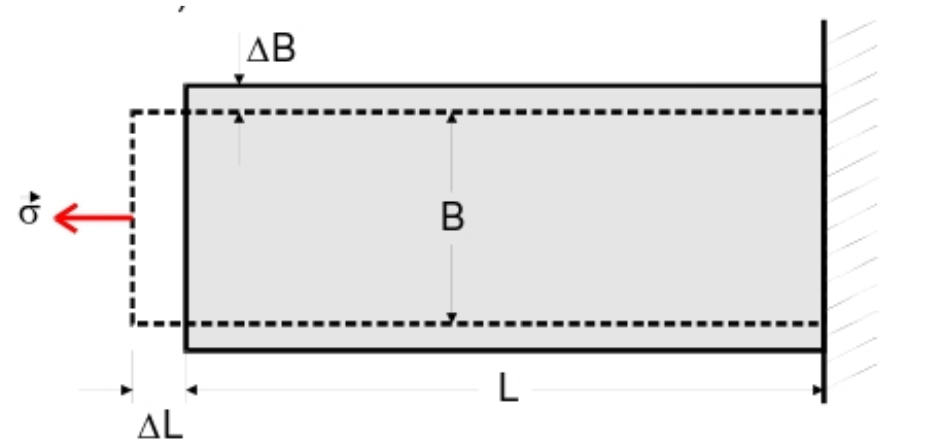
\includegraphics[width=5.0cm]{./picture/poisson.png}
  \caption{Längenänderung durch Normalspannung \cite{sample}.}
  \label{fig:poisson}
\end{figure}
\begin{equation}
  \mu := -\frac{\Delta B}{B} \cdot \frac{L}{\Delta L} = \frac{E}{2G} - 1
  \label{eqn:pois}
\end{equation}
Der Kompressionsmodul $Q$ berechnet sich aus dem Elastizitätsmodul so wie der Querkontraktionszahl $\mu$.
\begin{equation}
  Q = \frac{E}{-6 \mu + 3}
  \label{eqn:komp}
\end{equation}

\subsection{Bestimmung des Torsionsmoduls G}
Um die elastische Nachwirkung vernachlässigen zu können, wird zur Bestimmung des Torsionsmoduls eine dynamische Methode gewählt. Als elastische Nachwirkung wird die Zeit, die benötigt wird bis gewisse Materialien nach einer Belastung wieder in ihren Ausgangszustandung zurückgekehrt sind bezeichnet.
Für die dynamische Methode wird ein Draht an einem Ende eingespannt und auf der anderen Seite wirkt über ein Kräftepaar ein Drehmoment auf diesen. Durch die Scherung des Drahtes um den Winkel $\alpha$ kommt es zu einem Drehmoment. Dieses infinitesimale Drehmomente wird über den Radius des Zylinders integriert.
\begin{equation}
  M = \frac{\pi G R^4 \varphi}{2L} =: D \varphi
  \label{eqn:M}
\end{equation}
In Analogie zur Federkonstante wird $D$ als Richtgröße bezeichnet. Durch eine kleine Auslenkung aus der Ruhelage im Rahmen der Kleinwinkelnäherung lässt sich das Schwingungsfähige System durch die Differentialgleichung
\begin{equation}
  D \varphi + \theta \varphi = 0
  \label{eqn:dgl}
\end{equation}
beschreiben, wobei $\theta$ das Trägheitsmoment des Systems ist. Der Differentialgleichung wird eine Periodendauer von
\begin{equation}
  T = 2 \pi \sqrt{\frac{\theta}{D}}
  \label{eqn:T}
\end{equation}
entnommen und das Trägheitsmoment der Kugel aus der Formel
\begin{equation}
  \theta_\text{Kugel} = \frac{2}{5}m_\text{k}R_\text{k}^2
  \label{eqn:theta}
\end{equation}
berechnet. Somit ergibt sich aus Formel \ref{eqn:M}, \ref{eqn:T} und \ref{eqn:theta} ein Torsionsmodul $G$ von
\begin{equation}
  G = \frac{16 \pi m_\text{k} R_\text{k}^2 L}{5 T^2 R^4} \ .
  \label{eqn:G}
\end{equation}
\subsection{Magnetisches Moment eines Permanentmagnetens}
Das magnetische Moment $\vec{m}$ eines Permanentmagneten ist definiert als
\begin{equation}
  \vec{m} := p \vec{a}
  \label{eqn:m}
\end{equation}
wobei $p$ die Polstärke ist und $\vec{a}$ die Abstände der beiden Pole sind. Auf den Magneten wirkt in einem B-Feld wie in Abbildung \ref{fig:MagM} zu sehen,
\begin{figure}
  \centering
  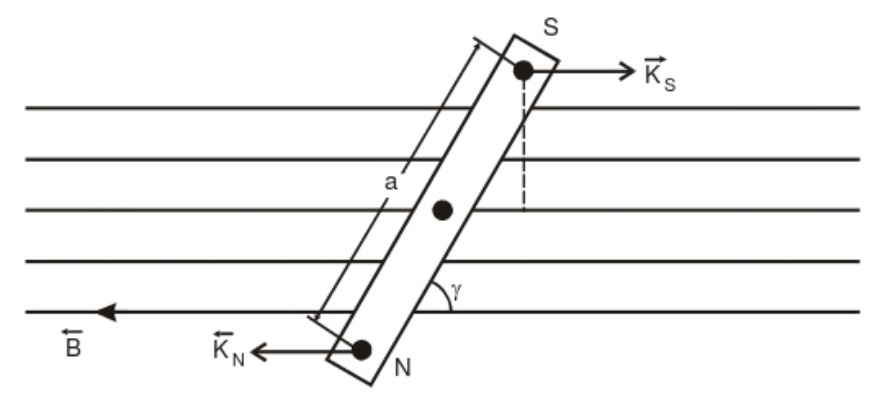
\includegraphics[height=6cm]{picture/MagM.png}
  \caption{Magnetisches Moment eines Permanentmagneten im B-Feld \cite{sample}.}
  \label{fig:MagM}
\end{figure}
dass magnetische Moment $M_\text{Mag}$ zweier entgegengesetzter Kräfte. Der Betrag des magnetischen Momentes ist
\begin{equation}
  |M_\text{Mag}| = m B \sin(\gamma) \ .
  \label{eqn:MM}
\end{equation}
Wird nun ein externes Magnetfeld hinzugeschaltet, wird die Gleichung (\ref{eqn:dgl}) mit dem zusätzlichen magnetischen Moment $M_\text{Mag}$ erweitert und es ergibt sich:
\begin{equation}
  mB \sin(\varphi) + D \varphi + \theta \frac{d^2 \varphi}{dt^2} = 0 \ .
  \label{eqn:idgl}
\end{equation}
Nun wird noch die Kleinwinkelnäherung $\sin \varphi \sim \varphi$ angewendet wodurch der sin wegfällt. Daraus lässt sich die Schwingungsdauer
\begin{equation}
  T_\text{Mag} = 2 \pi \sqrt{\frac{\theta}{mB + D}}
  \label{eqn:Tmag}
\end{equation}
entnehmen.
\subsection{Fehlerrechnung}
\subsubsection{Mittelwert}
Der Mittelwert einer Messreihe $x_\text{1}, ... ,x_\text{n}$ lässt sich durch die Formel
\begin{equation}
	\overline{x} = \frac{1}{N} \sum_{\text{k}=1}^\text{N} x_k
	\label{eqn:ave}
\end{equation}
berechnen. Die Standardabweichung des Mittelwertes beträgt
\begin{equation}
	\Delta \overline{x} = \sqrt{ \frac{1}{N(N-1)} \sum_{\text{k}=1}^\text{N} (x_\text{k} - \overline{x})^2}
	\label{eqn:std}
\end{equation}

\subsubsection{Fehlerfortpflanzung}
Die Fehlerfortpflanzung übernimmt Python 3.4.3 mit der Funktion "ufloat" aus "Python-Uncertainties".

\subsubsection{Lineare Regression}
Die Lineare Regression und sämtliche andere Rechnungen wurden ebenfalls mit Python 3.4.3 durchgeführt.
